\documentclass[a4paper,fleqn]{cas-dc}
\usepackage[numbers]{natbib}
\usepackage{lipsum}

\def\tsc#1{\csdef{#1}{\textsc{\lowercase{#1}}\xspace}}
\tsc{WGM}
\tsc{QE}


\begin{document}

\title [mode = title]{The"Resus:Station": The use of clinical simulations in
a randomised crossover study to evaluate a novel resuscitation trolley}  

\shorttitle{A Spanish translated version of the
abstract of this article appears}    

% First author
\author[1]{Susanna T. Walkera}[type=editor,
       style=chinese,
       auid=000,
       bioid=1,
       prefix=Sir,
       orcid=0000-0000-0000-0000,
       facebook=facebook id,
       twitter=twitter id,
       linkedin=linkedin id,
       gplus=gplus id]
       
\ead{email address}

% Credit authorship
% eg: \credit{Conceptualization of this study, Methodology, Software}
\credit{Credit authorship details}

% Address/affiliation
\affiliation[1]{organization={Charles Vincenta linical Safety Research Unit},
       addressline={Department of Surgery  Cancer, mperial Colege london,10th Floor 0EOM Building, St Mary's Hospital, Praed Street}, 
            city={London},
            postcode={300200}, 
          state={NYUKb},
            country={USA}
}


\begin{abstract}
\emph{Background and aim:} lnadequately designed equipment has been implicated in poor efficiency and criticalincidents associated with resuscitation. A novel resuscitation trolley (Resus:Station) was designed ancevaluated for impact on team efficiency, user opinion, and teamwork, compared with the standard trolleyin simulated cardiac arrest scenarios.

\emph{Methods:} Fifteen experienced cardiac arrest teams were recruited (45 participants). Teams performedrecorded resuscitation simulations using new and conventional trolleys, with order of use randomised.

After each simulation, efficiency (“time to drugs", un-locatable equipment, unnecessary drawer open-ing) and team perforance (OSCAR) were assessed from the video recordings and participants wereasked to complete questionnaires scoring various aspects of the trolley on a Likert scale.Results: Time to locate the drugs was significantly faster (p =0001) when using the Resus:Station (mean5.19 s(SD 3.34)) than when using the standard trolley (26.81 s (SD16.05)).

There were no reports of missing equipment when using the Resus:Station. However, during four ofthe fifteen study sessions using the standard trolley participants were unable to find equipment, with anaverage of 6.75 unnecessary drawer openings per simulation.

User feedback results clearly indicated a highly significant preference for the newly designedResus:Station for all aspects.

Teams performed equally well for all dimensions of team performance using both trolleys, despite itbeing their first exposure to the Resus:Station.Conclusion: We conclude that in this simulated environment, the new design of trolley is safe to use, andhas the potential to improve efficiency at a resuscitation attempt.


\end{abstract}


\begin{keywords}
Resuscitation trolley\sep
Clinical simulation\sep
Patient safety\sep
Equipment design\sep
Team efficiency
\end{keywords}

\maketitle


\section{Introduction}
\label{Intro}

\lipsum[1-7]


\begin{figure*}[t]
	\centering
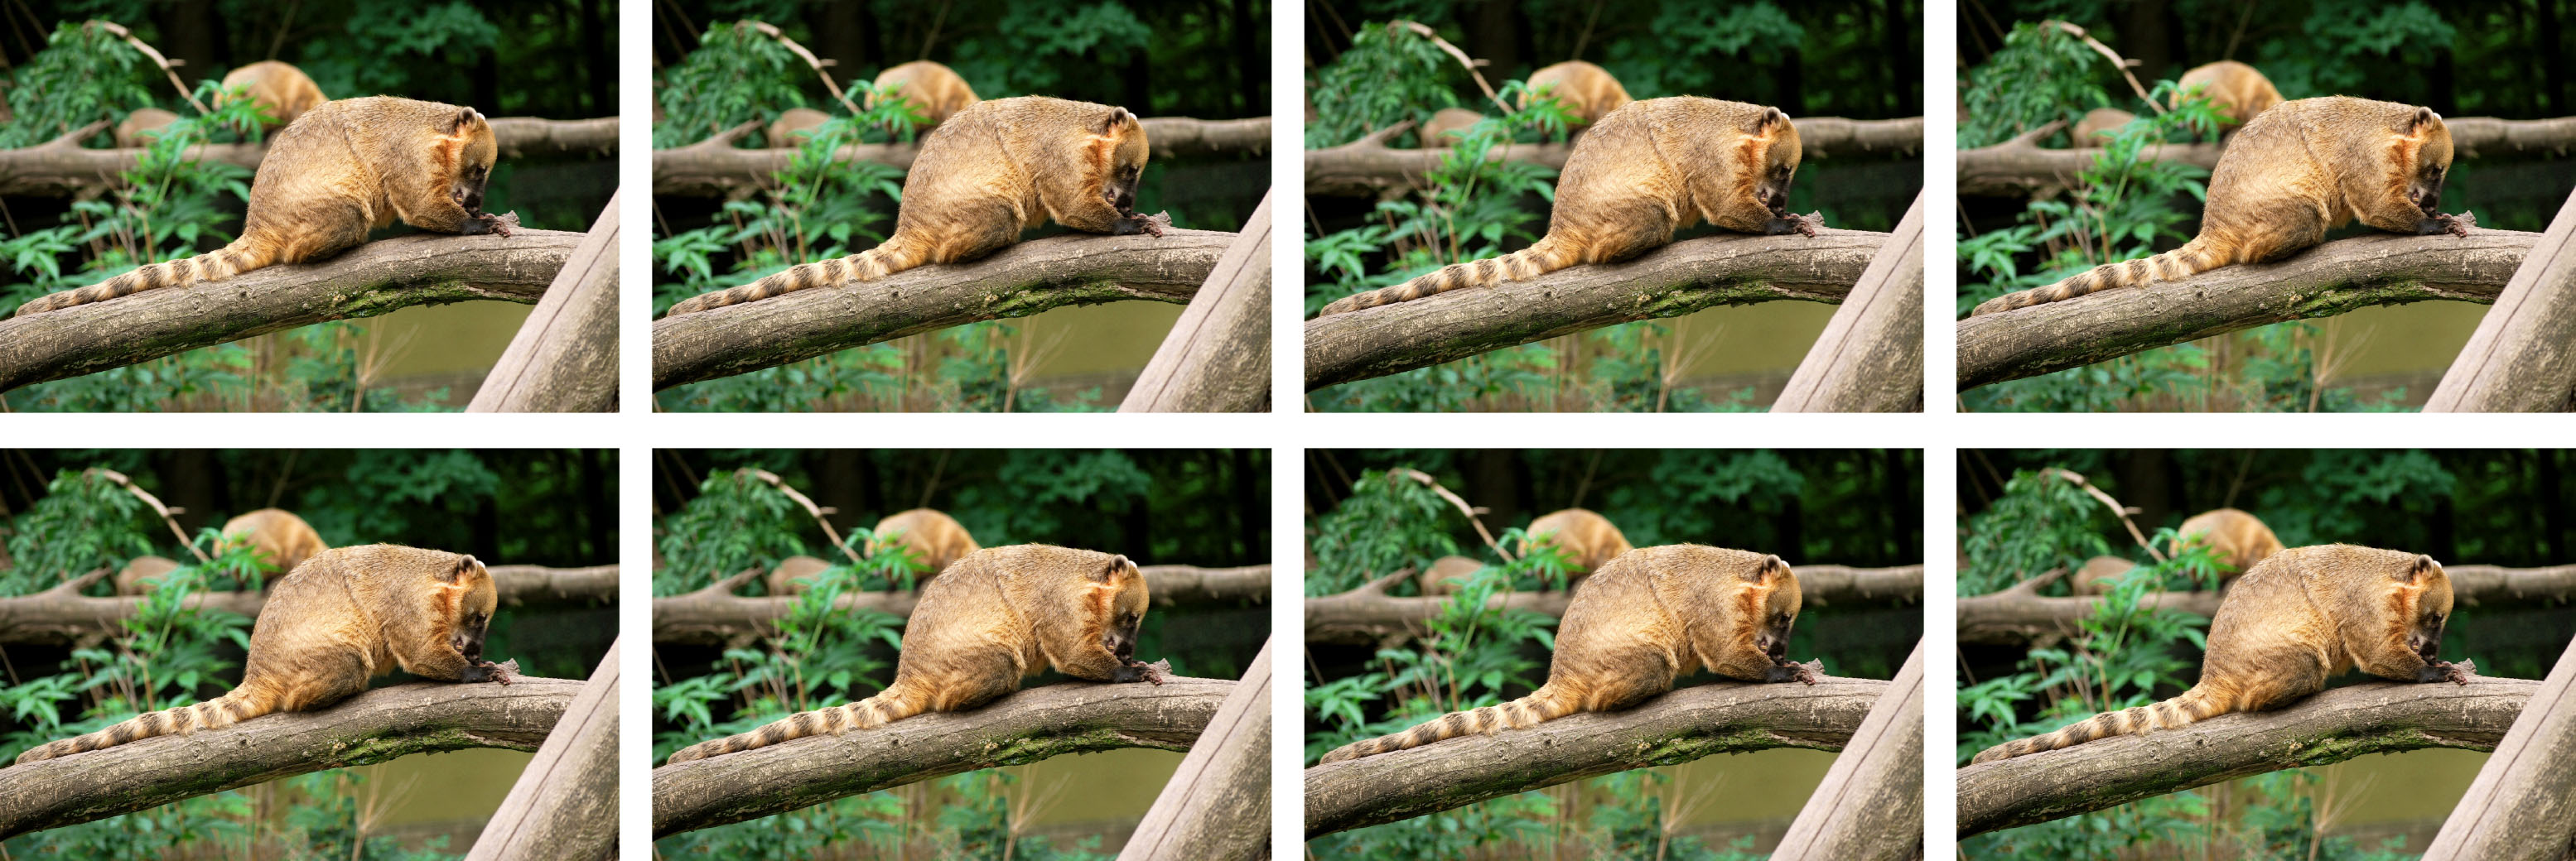
\includegraphics[width=\textwidth]{fig1-2}
	  \caption{The main limitation of this study is that the small cardiac arrestteam, and short simulation scenario limited the possibilities for effi-ciency assessment. We would ideally repeat this at a real arrest witha full resuscitation team. However, this small study has enabled usto have some insight into the potential impact of an ergonomicallydesigned resuscitation trolley.}
\label{fig1}
\end{figure*}


\section{Methods}
\label{Methods}

\begin{figure*}[b]
	\centering
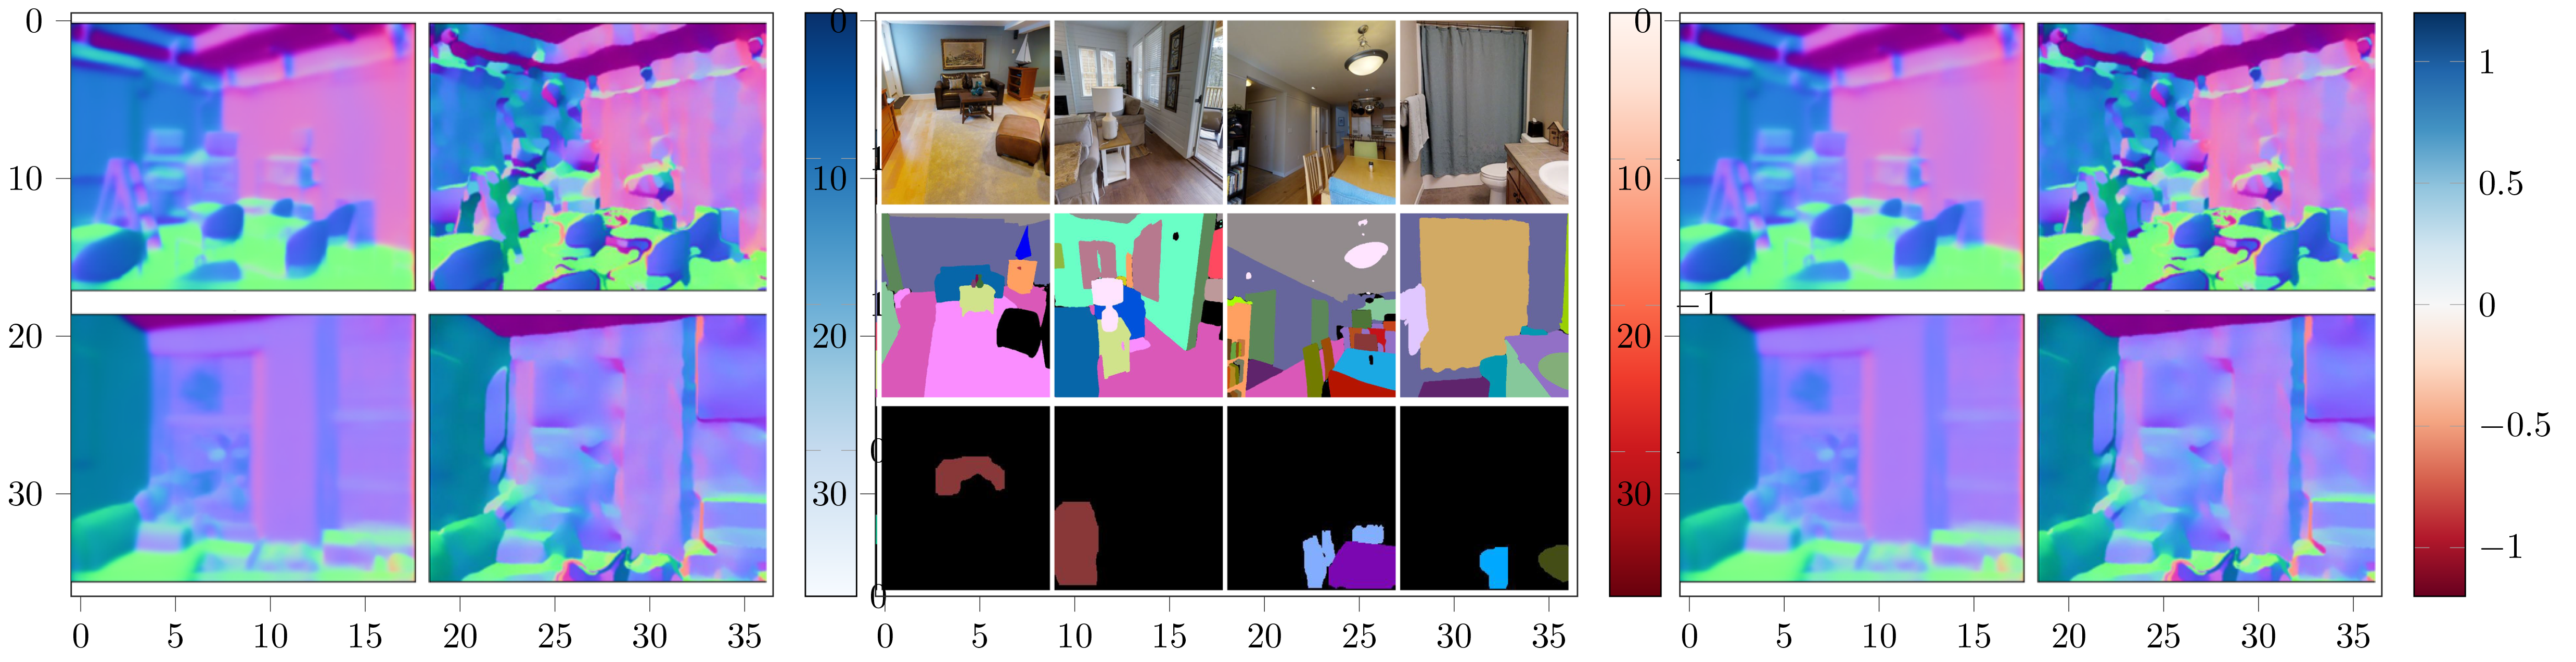
\includegraphics[width=\textwidth]{fig2}
	  \caption{Quisque ullamcorper placerat ipsum. Cras nibh. Morbi
vel justo vitae lacus tincidunt ultrices. Lorem ipsum dolor
sit amet, consectetuer adipiscing elit. In hac habitasse platea
dictumst. Integer tempus convallis augue. Etiam facilisis.
Nunc elementum fermentum wisi. Aenean placerat. Ut im-
perdiet, enim sed gravida sollicitudin, felis odio placerat
quam, ac pulvinar elit purus eget enim. Nunc vitae tortor.
Proin tempus nibh sit amet nisl. Vivamus quis tortor vitae
risus porta vehicula.}
\label{fig1}
\end{figure*}

\lipsum[1-7]

\section{Results}
\label{Results}

\lipsum[1-7]

\end{document}

